\documentclass{article}
\usepackage{biblatex} %Imports biblatex package
\addbibresource{refs.bib} %Import the bibliography file
\usepackage{float, booktabs}
\usepackage[newfloat]{minted}
\usepackage{caption}
\usepackage{wrapfig}
\usepackage{subfig}
\usepackage{forest}
\usepackage{url}
\usepackage[utf8]{inputenc}
\setlength\parindent{0pt}
\usepackage{parskip} 
\usepackage{geometry}
 \geometry{
 a4paper,
 total={170mm,257mm},
 left=20mm,
 right=20mm,
 top=20mm,
 bottom=20mm,
 }
 \usepackage{graphicx}
 \usepackage{titling}
 \usepackage{amsmath,amsfonts,amssymb,amsthm,float}

\newenvironment{code}{\captionsetup{type=listing}}{}
\SetupFloatingEnvironment{listing}{name=Source Code}

\title{RNA-Seq Data Analysis of Bipolar Disorder}
\author{Dohyoung Ko}
\date{December 15 2024}
 
 \usepackage{fancyhdr}
\fancypagestyle{plain}{%  the preset of fancyhdr 
    \fancyhf{} % clear all header and footer fields
    \fancyfoot[L]{\thedate}
    \fancyfoot[R]{Page \thepage \hspace{1pt}}
    \fancyhead[L]{Genomic Data Science Final Project}
    \fancyhead[R]{\theauthor}
}
\makeatletter
\def\@maketitle{%
  \newpage
  \begin{center}%
  \let \footnote \thanks
    {\huge \@title \par}%
    \vskip 2em%
    {\large Dohyoung Ko, Akshay Nataraja}%
    \vskip 1em%
    {Department of Computer Science and Engineering, The Pennsylvania State University}
    \vskip 1em%
    {\@date}
  \end{center}%
  \par
  \vskip 1em}
\makeatother

\usepackage{cmbright}
\renewcommand{\epsilon}{\varepsilon}
\newcommand{\abs}[1]{\left\lvert #1 \right\rvert} % absolute value 
\newcommand{\bF}{\mathbb{F}}
\newcommand{\bD}{\mathbb{D}}
\newcommand{\bR}{\mathbb{R}}
\newcommand{\bN}{\mathbb{N}}

\begin{document}

\renewcommand{\theFancyVerbLine}{
  \sffamily\textcolor[rgb]{0.5,0.5,0.5}{\scriptsize\arabic{FancyVerbLine}}}


\maketitle

\section*{\centering Abstract}
This thesis presents a comprehensive analysis of RNA-Seq data to investigate the molecular underpinnings of bipolar disorder (BD), alongside the implementation of a computational pipeline optimized for high-performance computing (HPC) environments. The pipeline performs a robust and systematic analysis of raw Illumina high-throughput RNA-Seq reads, ensuring efficient and accurate data processing. The study outlines the rationale, methodology, and implementation details of each step in the RNA-Seq data analysis workflow. RNA-Seq data from the human dorsal striatum were utilized to profile transcriptomes, comparing cohorts of bipolar disorder patients to healthy controls. Differential gene expression (DGE) analysis was conducted using the \texttt{DESeq2} library to identify genes exhibiting significant changes in expression associated with bipolar disorder status. The results were further analyzed to uncover sets of co-expressed and correlated genes, providing insights into their potential association with bipolar disorder.

\hfill

\tableofcontents

\pagebreak

\section{Data Analysis Workflow}
This section provides a comprehensive overview of the computational pipeline developed for RNA-Seq data analysis, focusing on the standard workflow for differential gene expression (DGE) analysis. Given the raw sequencing reads stored in \texttt{FASTQ} files, RNA-Seq data analysis proceeds through several computational stages, each designed to process, align, and quantify the data systematically. While there are multiple possible approaches to analyzing RNA-Seq data depending on the dataset and study design, for this analysis, we aligned short Illumina reads to the reference genome to ensure robust and biologically relevant results. The overall workflow adopted for DGE analysis is depicted in Figure~\ref{fig:dgea_workflow}.
\begin{figure}[H]
    \centering
    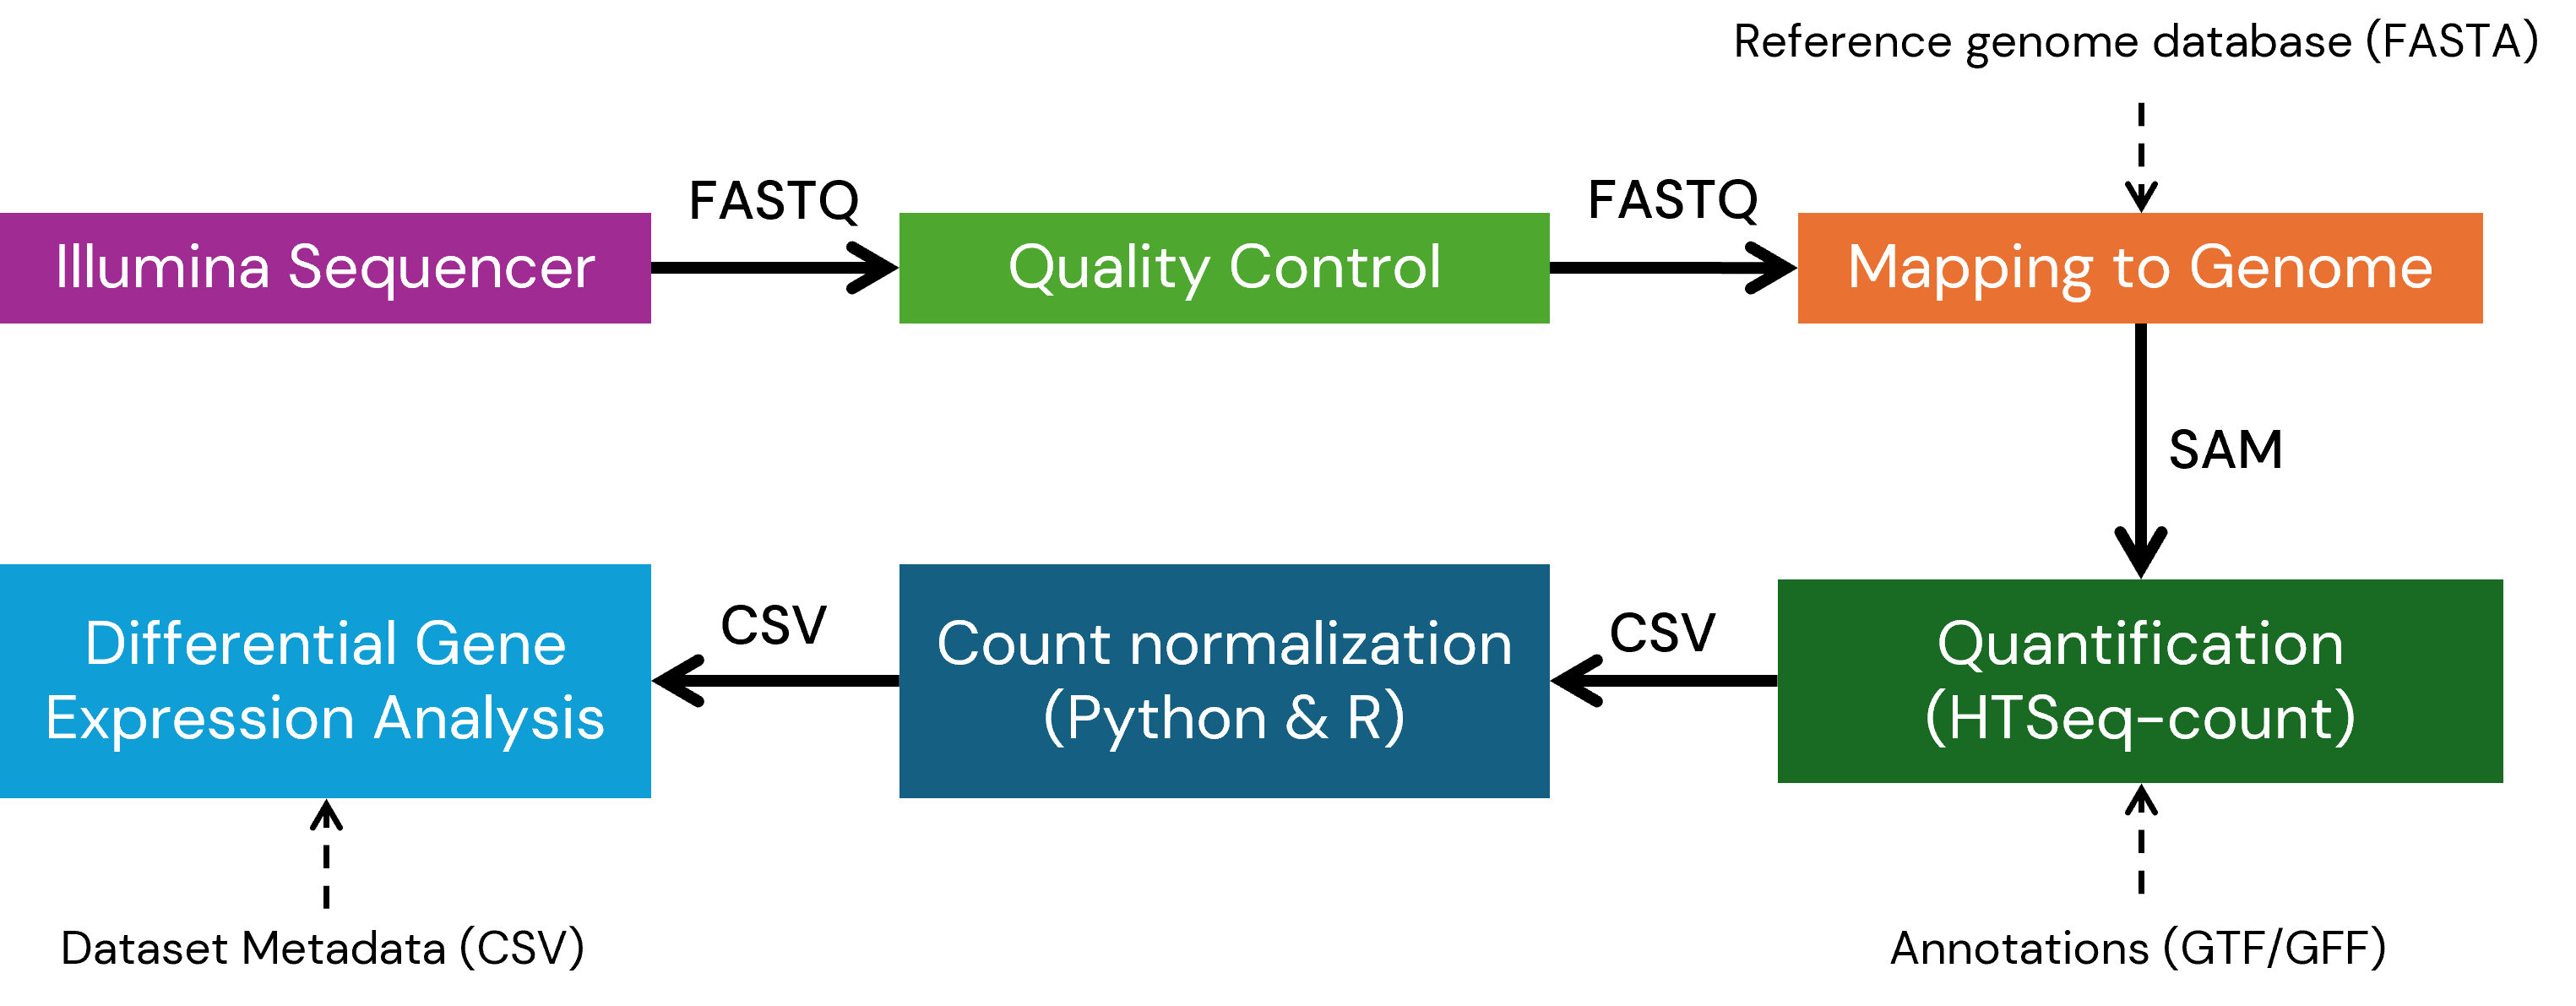
\includegraphics[width=0.8\linewidth]{workflow_img/dgea_workflow.png}
    \caption{Workflow of Differential Gene Expression Analysis}
    \label{fig:dgea_workflow}
\end{figure}
As a preliminary step, the raw Illumina sequencing reads encoded in \texttt{FASTQ} files were pre-processed to ensure high-quality data for downstream alignment and quantification. Pre-processing included demultiplexing reads based on indices or barcodes, removing residual adapter sequences introduced during library preparation, trimming bases with low quality scores, and discarding reads that were ambiguous or of insufficient quality. These steps are essential for minimizing alignment errors and ensuring the reliability of subsequent analyses.

The pre-processed reads were then aligned to the reference genome using HISAT2. HISAT2 begins by indexing the reference genome, which involves creating a hash table of short, non-overlapping substrings that facilitate efficient alignment. Each sequencing read is then scanned and mapped to its most likely genomic location by matching it against these indexed substrings. The output of the alignment step is a \texttt{SAM} (Sequence Alignment/Map) file.

The SAM file consists of two main sections: a header section and an alignment section. The header section, identified by lines starting with the \texttt{@} symbol, contains metadata about the alignment process. For instance, the \texttt{@HD} line specifies the file format version and the sorting order of alignments, while the \texttt{@SQ} lines define the reference sequences used during alignment. In these lines, the sequence name (\texttt{SN}) identifies each genomic feature (such as \texttt{NC\_000001.11}, representing chromosome 1), and the sequence length (\texttt{LN}) provides the total number of base pairs in that feature. The alignment section follows the header and contains detailed information for each mapped read, including its genomic position, mapping quality score, and additional aligner-specific parameters.

Once the reads were aligned, the next step involved quantifying gene expression levels by determining the number of reads that overlapped annotated genomic features. For this purpose, gene annotation data in \texttt{GTF} format was sourced from the NCBI \textit{Homo sapiens} genome database. This annotation file provides detailed genomic coordinates and attributes for features such as exons and genes, enabling precise quantification. The \texttt{htseq-count} tool was used to compute gene-level counts from the alignment data. \texttt{htseq-count} systematically compares each aligned read in the SAM file to the genomic features defined in the annotation file. Reads that overlap with a single genomic feature, such as an exon, are assigned to that feature, and mapped reads with overlapping multiple features are excluded to prevent miscounts. The resulting counts were aggregated at the gene level based on the \texttt{gene\_id} attribute specified in the annotation file. This step produced a raw count file in tabular format, where each row corresponds to a gene and its associated read count.

To prepare for downstream differential gene expression analysis, the count data for all cohort samples were combined into a single count matrix. This matrix was subsequently analyzed using the \texttt{DESeq2} library in \texttt{R}. \texttt{DESeq2} applies normalization and statistical modeling to identify genes with significant changes in expression levels between experimental groups. In this study, the comparison focused on cohorts of bipolar disorder patients and healthy controls, with the objective of identifying genes whose expression levels were significantly altered in association with bipolar disorder.

The results of the DGE analysis provided a list of differentially expressed genes, ranked according to their statistical significance and magnitude of expression change. These findings were further analyzed to identify sets of correlated or co-expressed genes.

\pagebreak

\section{Computational Pipeline}
This section discusses the design principles and implementation of the computational pipeline used to execute the RNA-Seq data analysis workflow described above. All computational processes were carried out on the Cedar heterogeneous computing cluster at Simon Fraser University, part of the Advanced Research Computing (ARC) service provided by the Digital Research Alliance of Canada. A single end-to-end execution of the pipeline took approximately 8 hours, utilizing 36 computing nodes with a total of 1,152 CPU cores and 800 gigabytes of memory on the Cedar cluster.

\subsection{Design and Specifications}
The computational pipeline, which streamlines the complete RNA-Seq differential gene expression (DGE) analysis process, is publicly available on GitHub at \url{https://github.com/Codakshay/RNA_Seq_Final_Project.git}. Designed as a command-line application, the pipeline offers an efficient, automated, and reproducible solution for high-performance computing (HPC) environments. It integrates multiple tools and processes seamlessly using the \texttt{slurm} workload manager and runs on Linux operating systems such as AlmaLinux 9 and CentOS 7.

The pipeline is implemented as a modular framework, combining Python, R, shell scripts, and a \texttt{Snakemake} workflow. By leveraging \texttt{Snakemake}, the pipeline allows task parallelization and efficient resource management across multiple compute nodes. This design significantly reduces processing time, making it suitable for large-scale RNA-Seq datasets.
\begin{table}[H]
\renewcommand{\arraystretch}{1.2} % Adjust the factor as needed
\centering
\begin{tabular}{ll}
\toprule
Operating System & Linux (AlmaLinux 9, CentOS 7) \\
Workload Management & slurm \\
Cores & minimum of 32 cores \\
Memory & minimum of 50 gigabytes + total size of FASTQ files \\
External Dependencies & python ($\geq$ 3.9.0), R ($\geq$ 4.0.5) \\
Estimated Processing Time & 24-48 hours depending on the FASTQ data size \\
\bottomrule
\end{tabular}
\caption{System Requirements}
\label{tab:system_requirements}
\end{table}
To ensure optimal performance and reproducibility, the pipeline adheres to the specifications outlined in Table~\ref{tab:system_requirements}. These requirements include the minimum number of CPU cores, memory size, and software dependencies necessary for the successful execution of the analysis. Depending on the size of the input \texttt{FASTQ} files, the estimated runtime for a complete analysis ranges between 24 and 48 hours.

By consolidating all steps of RNA-Seq data analysis into a single pipeline, this implementation provides an effective one-click solution for large-scale genomic studies in high performance computing (HPC) environments.

\subsection{Installation}
We recommend installing the pipeline directly from the GitHub repository to ensure access to the most recent version, including any updates or fixes. To install the pipeline on your computing cluster, execute the following command:

\begin{minted}{shell}
git clone https://github.com/Codakshay/RNA_Seq_Final_Project.git
\end{minted}
For all subsequent steps, ensure you navigate to the root directory of the cloned repository.

Before running the pipeline, it is essential to verify that your computing cluster supports both R and Python as available modules. Most high-performance computing (HPC) environments use module management systems (e.g., \texttt{module load}) to provide software packages. You should confirm that R (version $\geq 4.0.5$) and Python (version $\geq 3.9.0$) are accessible. If these are not pre-installed, contact your system administrator to install or enable them.

Additionally, ensure that all Python dependencies listed in the \texttt{requirements.txt} file located in the root directory of the repository are installed on the cluster. The required libraries can be installed locally in a virtual environment or within a Conda environment. To set up the environment and install the necessary libraries, execute the following commands:
\begin{minted}{shell}
python3 -m venv env source env/bin/activate pip install -r requirements.txt
\end{minted}
This will create an isolated virtual environment containing all the required Python dependencies for running the pipeline. If you encounter any issues, verify that the correct Python version is being used and that the required libraries are available.

\subsection{Running the Pipeline}
This subsection provides a concise manual for executing the computational pipeline on a high-performance computing (HPC) environment. Before proceeding, please verify that your computing system meets the design specifications outlined in the previous subsection.

The pipeline requires only a BioProject ID as input. At its current stage, the pipeline exclusively supports RNA-Seq differential gene expression analysis for Homo sapiens data. The necessary datasets, including raw sequencing reads and reference annotations, are automatically retrieved from the NCBI FTP server by the pipeline script, as illustrated in Figure~\ref{fig:ncbi-navigator}.
\begin{figure}[H]
    \centering
    \subfloat[\centering Search for BioProject ID on NCBI Database]{{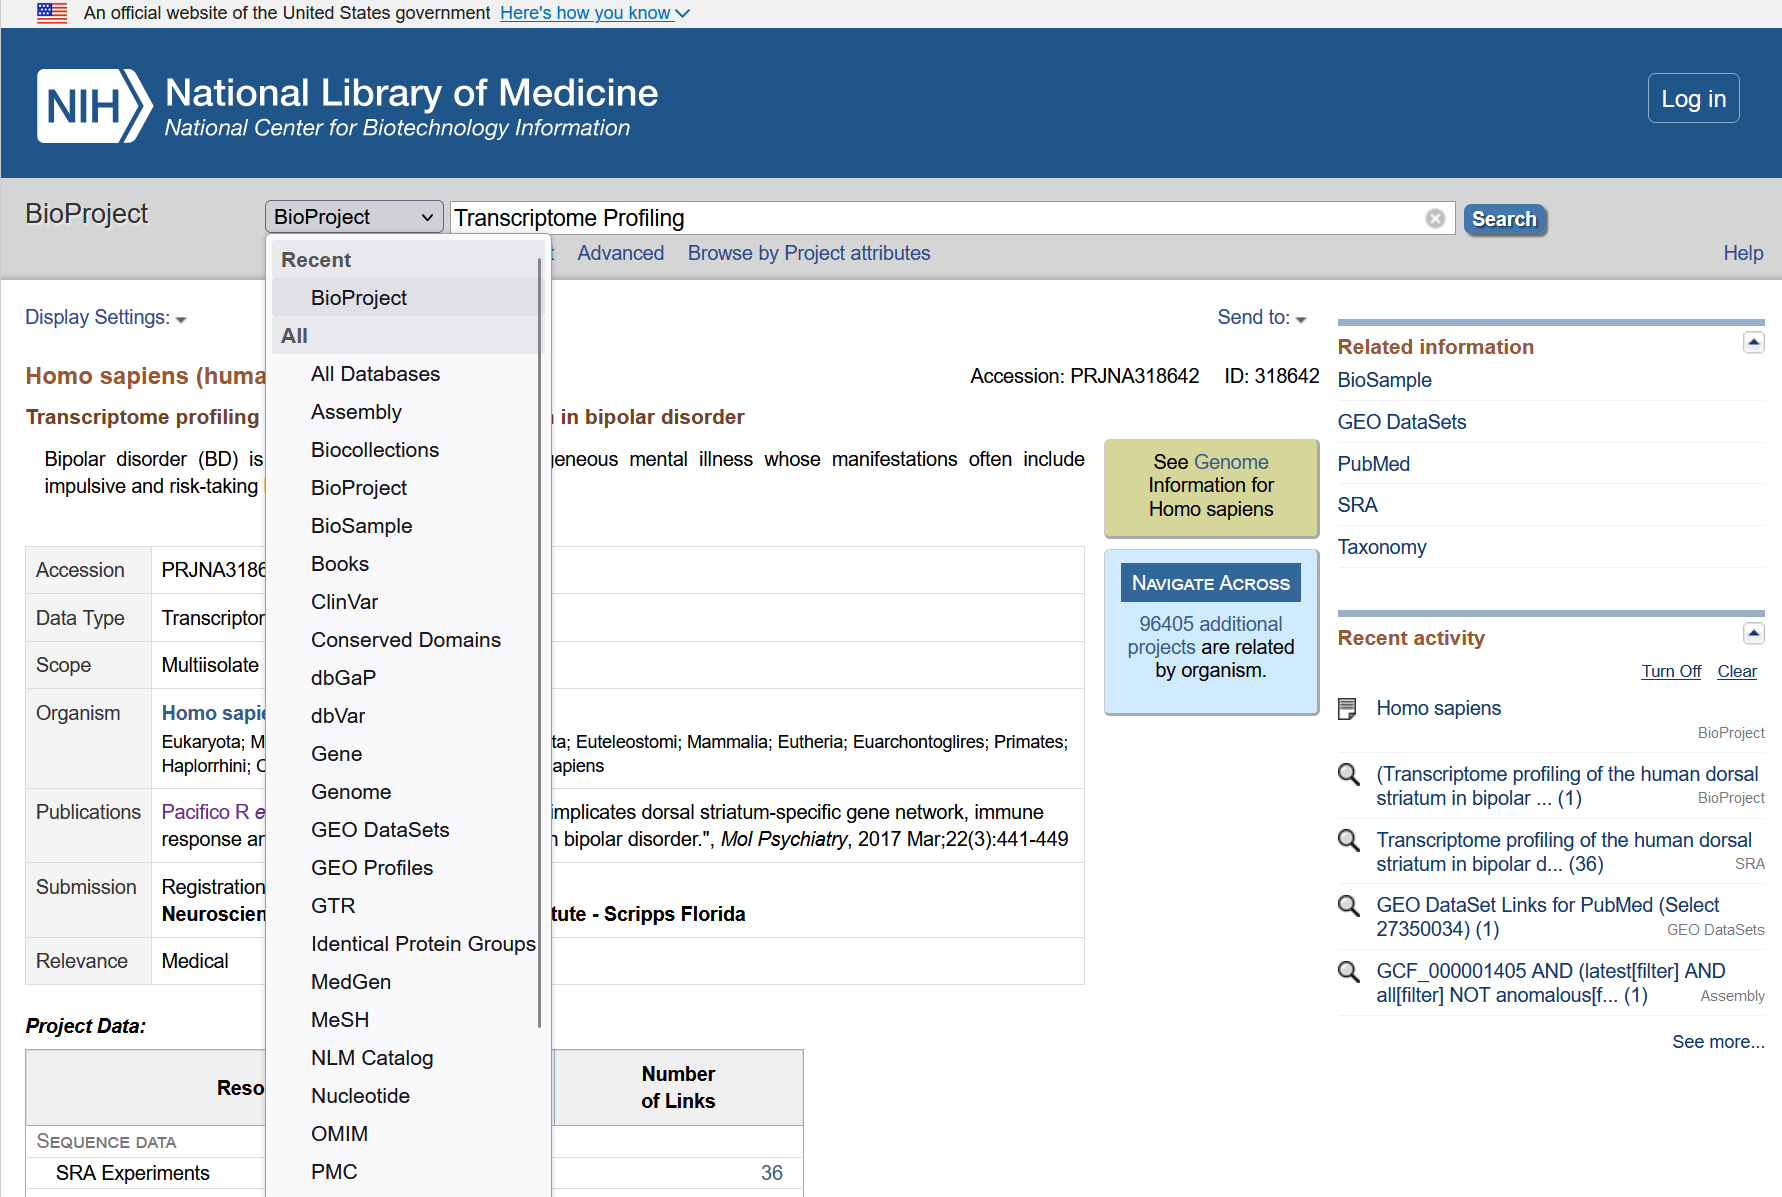
\includegraphics[height=5cm]{workflow_img/BioProjectID.png} }}%
    \qquad
    \subfloat[\centering Human Reference Genome in FASTA and GTF annotations]{{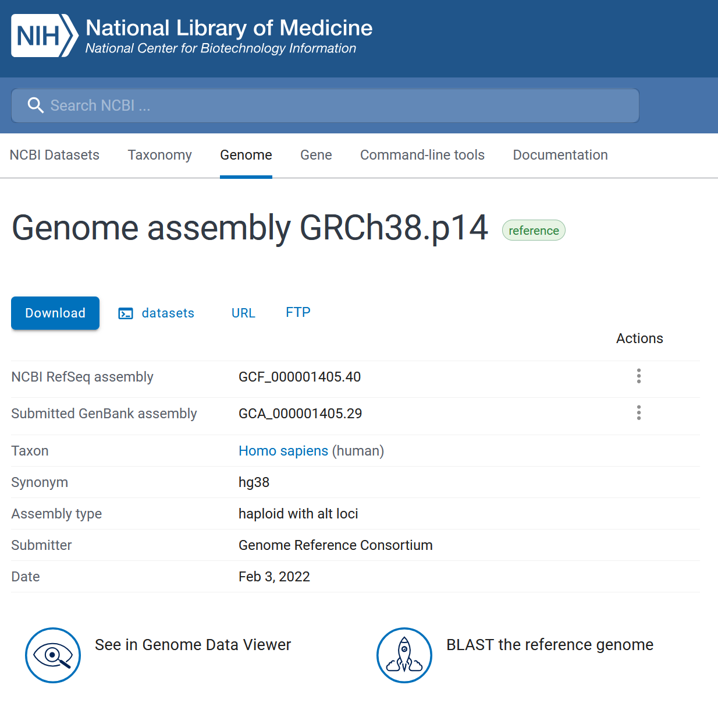
\includegraphics[height=5cm]{workflow_img/human_ref_genome.png}}}%
    \caption{BioProject ID and Human Reference Genome on NCBI Database}
    \label{fig:ncbi-navigator}
\end{figure}
This application requires only a BioProject ID as input. At its current stage, the pipeline exclusively supports RNA-Seq differential gene expression analysis for Homo sapiens datasets. The required sequencing data, including raw reads and associated annotations, are automatically retrieved from the NCBI FTP server by the pipeline script, as illustrated in Figure~\ref{fig:ncbi-navigator}(b). Future iterations of the pipeline will expand support to RNA-Seq datasets from additional species to enable broader applicability.

In the NCBI Sequence Read Archive (SRA) database, BioProject IDs provide unique identifiers for retrieving all raw sequencing datasets associated with a particular project. These identifiers are typically formatted as \texttt{PRJNA} followed by a series of digits. BioProject IDs can be located either via the Gene Expression Omnibus (GEO) database or by directly searching the NCBI database. As shown in Figure~\ref{fig:ncbi-navigator}, users can find the BioProject ID by selecting “BioProject” in the search criteria. Once the appropriate BioProject ID is retrieved, users must navigate to the root directory of the cloned pipeline repository and execute the following command on their computing cluster:
\begin{minted}{shell}
sbatch run_pipeline.sh PRJNA123456 24:00:00
\end{minted}
In this command, \texttt{PRJNA123456} represents the BioProject ID, and \texttt{24:00:00} specifies the maximum expected execution time in \texttt{HH:MM:SS} format. While the total processing time depends on the number of \texttt{FASTQ} files and their sizes, typical runtimes range between 24 and 48 hours. For the case study conducted in this work, the pipeline completed execution in approximately 12 hours.

It is important to note that if the specified time limit is insufficient, the job will be automatically terminated by the SLURM workload manager. In such cases, the pipeline must be re-executed with an increased time allocation. Users are advised to monitor the execution status of their job by running the \texttt{sq} command, which provides real-time updates on job progress within the computing cluster.

While the execution process itself does not require user intervention, the status and potential errors can be monitored by inspecting the \texttt{.out} and \texttt{.err} files generated in the \texttt{RNA\_Seq\_Final\_Project/logs/} directory. These log files provide detailed information about the ongoing pipeline execution, including standard outputs and any error messages encountered during runtime.

\subsection{Retrieving Results}
Upon successful execution of the pipeline, the output consists of the results of the Differential Gene Expression (DGE) analysis along with all intermediate data objects generated during processing. This subsection describes the structure of the output files and directories, providing an overview of how the results are organized. The directory structure after pipeline execution is illustrated in the file tree diagram on the right.

\begin{wrapfigure}{r}{6cm}
\begin{forest}
for tree={
    font=\ttfamily,
    grow'=0,
    child anchor=west,
    parent anchor=south,
    anchor=west,
    calign=first,
    edge path={
        \noexpand\path [draw, \forestoption{edge}]
        (!u.south west) -- +(-5pt,0) |- (.child anchor)\forestoption{edge label};
    },
    before typesetting nodes={
        if n=1
            {insert before={[,phantom]}}
            {}
    },
    fit=band,
    before computing xy={l=15pt},
}
[RNA\_Seq\_Final\_Project
    [alignment
        [SRR12345678.sam]
    ]
    [data
        [plots
            [VolcanoPlot.png]
        ]
        [reference\_genome.fasta]
        [annotation.gtf]
    ]
    [fastq\_files
        [SRR12345678.fastq]
    ]
    [logs
        [job\_num\_192743123.out]
        [job\_num\_192743123.err]
    ]
    [ref\_genome
        [ref\_gen.ht2]
    ]
    [transcripts
        [counts\_SRR12345678.csv]
    ]
]
\end{forest}
\end{wrapfigure}
All preprocessed data, intermediate files, and final DGE analysis results are stored within the root directory of the pipeline. The key directories and their contents are as follows:

The \texttt{alignment} directory contains the SAM files generated by the HISAT2 alignment tool. These files store the processed alignments of the input sequencing reads (in \texttt{FASTQ} format) to the reference genome.

The \texttt{data} directory serves as the repository for processed data and results relevant to downstream analyses. It includes two primary components: the \texttt{plots} subdirectory, which contains visualizations such as volcano plots produced during DGE analysis, and the reference files used for alignment. Specifically, the directory includes the reference genome in \texttt{FASTA} format and its corresponding annotation file in \texttt{GTF} format. Both files are retrieved from the NCBI FTP server and are essential for mapping and quantifying sequencing reads.

The \texttt{fastq\_files} directory houses the raw input sequencing data in \texttt{FASTQ} format, which is downloaded directly from the NCBI SRA database based on the provided BioProject ID. This organization facilitates easy access to the original data and supports reproducibility.

The \texttt{logs} directory systematically stores all workflow logs, including job-specific output (\texttt{.out}) and error (\texttt{.err}) files generated during pipeline execution.

The \texttt{ref\_genome} directory contains the indexed reference genome files required by the HISAT2 aligner. These preprocessed reference files are used during alignment to map sequencing reads to genomic coordinates.

Finally, the \texttt{transcripts} directory holds the gene expression count files in \texttt{CSV} format. Each file corresponds to a cohort sample from the analysis and contains raw read counts for individual genes. These counts serve as the input for the downstream DGE analysis, where statistical tools such as \texttt{DESeq2} are used to identify genes with significant changes in expression between experimental conditions.

\newpage

\section{Dataset Analysis}
The subsequent analysis in the report employs the RNA-Seq dataset of the human dorsal striatum, which is comprised of 18 cohorts of individuals diagnosed with Bipolar Disorder (BD) and 18 control subjects.
\subsection{Origin and Context of DataSet}
As stated by R. Pacifico and RL Davis in \cite{pacifico2017transcriptome}, the data is derived from 36 frozen postmortem human striatum samples provided by the Harvard Brain Tissue Resource Center. These samples are accompanied by information regarding the age, sex, and postmortem interval (PMI) of sample collection from the donors. The original study excluded one outlier control sample, designated as C 28, and conducted differential gene expression (DGE) analysis on 35 samples (18 bipolar and 17 control). The covariates (age, sex, PMI, and RIN) for both the bipolar and control groups were not significantly different from each other. This report presents two results: one considering the inclusion of the C 28 control sample and another considering its exclusion. The objective is to observe the differences in the outcome of the DGE analysis. In bipolar disorder, it is especially important to consider how long the manic episode continues, and the data has been normalized to account for this constraint.
\begin{table}[H]
\centering
\begin{tabular}{llrlrr}
\toprule
geo accession & title & age (years) & Sex & postmortem interval (hours) & rin \\
\midrule
GSM2124738 & control-2 & 83 & male & 13.000000 & 3.700000 \\
GSM2124739 & control-3 & 55 & female & 21.660000 & 2.900000 \\
GSM2124771 & bipolar-34 & 80 & female & 13.660000 & 3.600000 \\
GSM2124772 & bipolar-37 & 61 & female & 16.630000 & 2.200000 \\
GSM2124773 & bipolar-40 & 77 & female & 29.580000 & 6.700000 \\
\bottomrule
\end{tabular}
\caption{Part of sampled cohort data}
\label{tab:metadata_entr}
\end{table}
Table \ref{tab:metadata_entr} refers to a part of the cohort data, which provides a more concrete description of the dataset.
\begin{table}[H]
\centering
\begin{tabular}{ccccc}
\toprule
Group & Age ($\mu \pm \sigma$) & Sex (Male, Female) & PMI ($\mu \pm \sigma$) & RIN ($\mu \pm \sigma$) \\
\midrule
Control & 65 $\pm$ 15.7 & 7, 11 & 22.8 $\pm$ 6.4 & 4 $\pm$ 1.7 \\
Cohort & 69.7 $\pm$ 15.3 & 6, 12 & 25.1 $\pm$ 15.8 & 3.9 $\pm$ 1.5 \\
\bottomrule
\end{tabular}
\caption{Summary of cohorts}
\label{table:cohort_info}
\end{table}
\noindent Table \ref{table:cohort_info} presents a summary of the most notable statistics from the dataset pertaining to each cohort and control group. It should be noted that these statistics exclude the effect of an outlier, C\_28, from the sample.

\subsection{Data Preprocessing}
This section outlines the specific data preprocessing operations required for RNA-Seq data analysis, as introduced earlier in the workflow overview. The preprocessing phase begins with handling the Illumina high-throughput sequencing data.

\subsubsection{Illumina RNA Sequencing Data}
RNA-Seq data is generated by sequencing RNA molecules extracted from a biological sample, followed by computational processing to reconstruct and quantify the transcriptome. The RNA-Seq workflow typically begins with the extraction of RNA from the biological sample, followed by its conversion into complementary DNA (cDNA) via reverse transcription. The resulting cDNA is then sequenced using high-throughput sequencing technologies. Illumina sequencing platforms, such as the HiSeq-2000, are among the most widely used technologies for this purpose. They provide high accuracy, throughput, and cost-efficiency, making them ideal for large-scale transcriptome studies.

RNA-Seq data can be generated using two primary sequencing strategies: single-end and paired-end sequencing. Single-end sequencing reads a fragment of the cDNA molecule from one end, while paired-end sequencing generates reads from both ends of the fragment, improving alignment accuracy and coverage. The high-throughput sequencing dataset used in this analysis consists of reads generated by the Illumina HiSeq-2000 platform.

Figure~\ref{fig:hiseq_machine} illustrates the process of obtaining RNA-Seq data from an RNA sample using the Illumina HiSeq-2000. In Figure~\ref{fig:hiseq_machine}(a), RNA extracted from a biological sample is sequenced to produce raw reads. Figure~\ref{fig:hiseq_machine}(b) shows the Illumina HiSeq-2000 machine used for sequencing, which is capable of producing millions of short reads in a single sequencing run.
\begin{figure}[H]
    \centering
    \subfloat[\centering Sequencing the RNA sample on Illumina HiSeq-2000]{{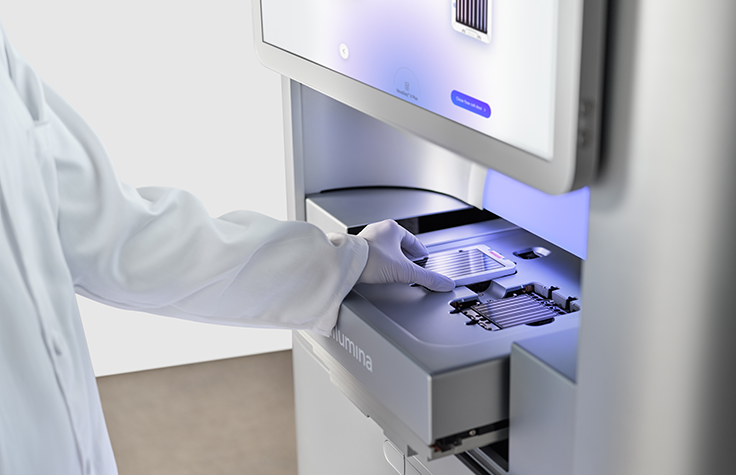
\includegraphics[width=7cm]{workflow_img/seq-illumina-technology.png} }}%
    \qquad
    \subfloat[\centering Illumina HiSeq-2000 Sequencing Machine]{{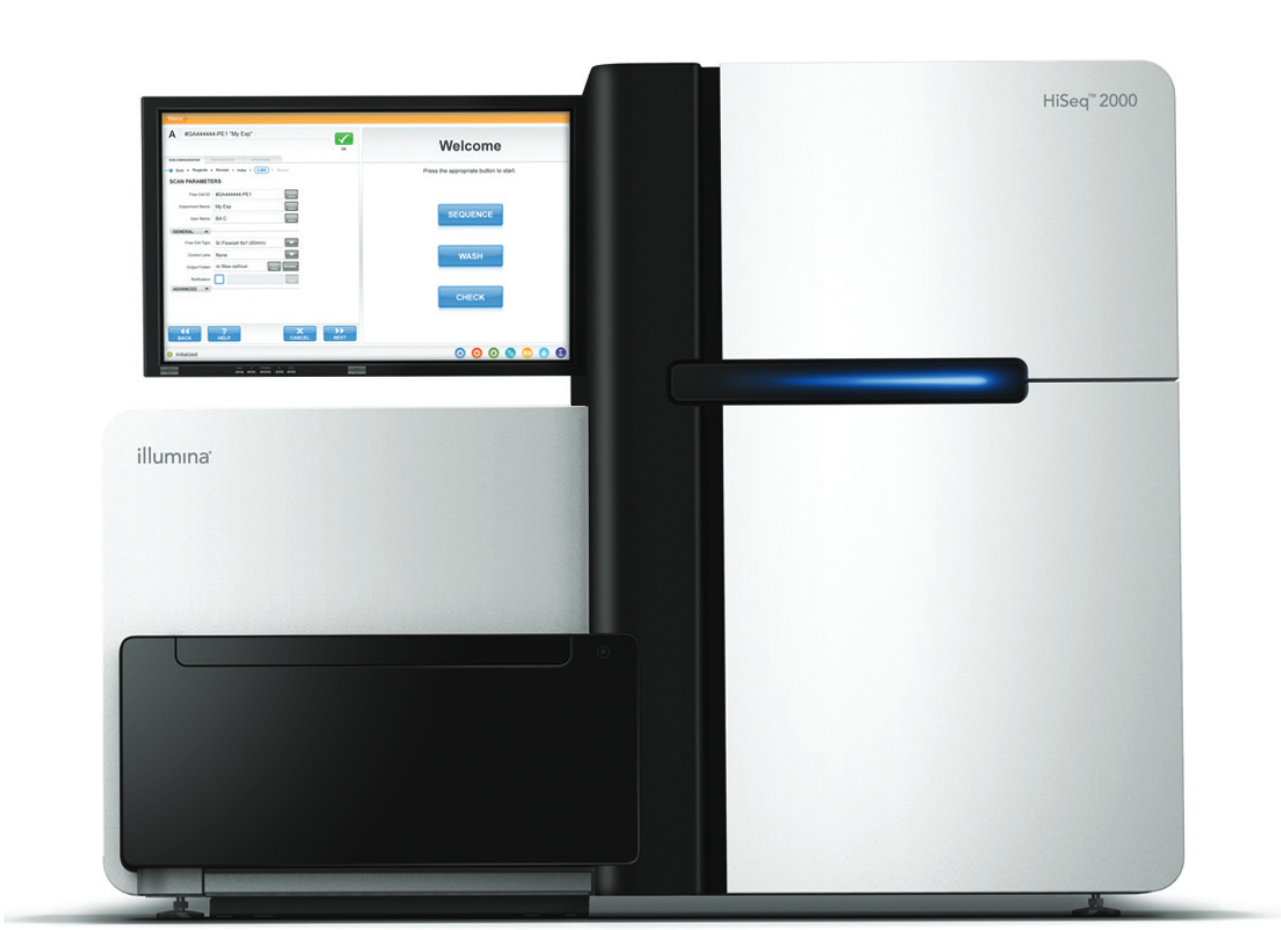
\includegraphics[width=7cm]{workflow_img/illumina-hiseq-3000.png}}}%
    \caption{High-throughput sequencing machine}
    \label{fig:hiseq_machine}
\end{figure}
In most cases, the raw RNA-Seq data is available in the FASTQ format. The following code section \ref{code:sample-fastq} describes the typical FASTQ file of RNA-Seq data.
\begin{code}
\captionof{listing}{Sample FASTQ output}
\label{code:sample-fastq}
\begin{minted}{ada}
@SRR3393492.1 HISEQ:313:D2H4NACXX:2:1101:1200:1867 length=88
NTCCGTCTTGCGCCGGGCCAAGAATTTCACCTCTAGCGGCGCAATACGAATGCCCCCGGCCGGCCCTCTTAATCATGGCCTCAGTTCC
+SRR3393492.1 HISEQ:313:D2H4NACXX:2:1101:1200:1867 length=88
#11?7?;AAACCACAA)??ABA3>AAAB0=ABBB<A><AA################################################
\end{minted}
\end{code}
Each record in a FASTQ file consists of four lines, which are repeated for every sequence in the file. The above data represents a single record. The first line begins with @ and serves as the sequence identifier, providing a unique name for the read (\texttt{SRR3393492.1}) and additional metadata such as sequencing instrument (\texttt{HISEQ:313:D2H4NACXX}) and read length (\texttt{length=88}). The second line contains the raw nucleotide sequence (\texttt{NTCCGTCTTGCGCCGGGCCAAGAATT...}), representing the biological data obtained from the sequencing process. The third line starts with a + symbol and may either repeat the sequence identifier or remain blank, serving as a separator for the quality scores. The fourth line encodes the quality scores using ASCII characters (\texttt{\#11?7?;AAACCACAA)...}), which represent Phred scores for each nucleotide.

The Phred score is a numerical value used to represent the quality of a nucleotide base call. It is a logarithmic measure of the probability \(P\) that a base call is incorrect. Higher Phred scores indicate higher confidence in the accuracy of the base call. Given that \(P\) is the probability of the base call being incorrect, its Phred score \(Q = -10 \log_{10}(P)\) is computed and encoded into an ASCII character by adding \(33\) to it. For instance, the character \(I\), which corresponds to ASCII 73, indicates a Phred score of 40.

Our computational pipeline downloads all FASTQ files from the NCBI SRA database. These raw sequencing data is then assembled into SAM files via HISAT2.

\subsubsection{Sequence Alignment Data}  
Before performing the sequence alignment, it is essential to construct the reference genome database, which serves as the base for aligning sequencing reads. The computational pipeline generates the reference genome database from the NCBI *Homo sapiens* reference genome dataset using the following command:

\begin{minted}{shell}
    hisat2-build -p 32 "data/GCF_000001405.40_GRCh38.p14_genomic.fna" "ref_genome/ref_gen"
\end{minted}

In this command, \texttt{hisat2-build} creates index files necessary for alignment using 32 parallel threads (\texttt{-p 32}). The input file is the reference genome in \texttt{.fna} format, while the output consists of indexed files stored under the specified prefix \texttt{ref\_genome/ref\_gen}. These index files allow efficient alignment of sequencing reads to the reference genome.

Once the reference genome database has been constructed, the pipeline proceeds with the alignment of sequencing reads (in \texttt{FASTQ} format) against the reference genome using HISAT2. The following command is executed:

\begin{minted}{shell}
hisat2 -p 32 -x ref_genome/ref_gen -U "fastq_files/SRR3393492.fastq" \
       -S "alignment/SRR3393492.sam"
\end{minted}
In this alignment step, \texttt{-p 32} specifies the use of 32 threads for multi-threaded processing. The tag \texttt{-x} points to the prefix of the reference genome index files created in the previous step. Also, \texttt{-U} specifies the input file containing single-end sequencing reads (\texttt{SRR3393492.fastq}). Finally, \texttt{-S} indicates the output file path, where the alignment results are stored in SAM (Sequence Alignment/Map) format.

The resulting SAM file contains essential information for each aligned read, including its position on the reference genome, alignment flags, mapping quality scores, and more. The header section of the SAM file provides metadata about the reference genome sequences used during alignment. Table~\ref{table:sam_header} shows the first few rows of the header section from the processed SAM file corresponding to cohort ID \texttt{SRR3393492}.
\begin{table}[H]
    \centering
    \begin{tabular}{cll}
        \toprule
        Record Type & Sequence Name (SN) & Sequence Length (LN) \\
        \midrule
        @SQ & NC\_000001.11 & 248956422 \\
        @SQ & NT\_187361.1 & 175055 \\
        @SQ & NT\_187362.1 & 32032 \\
        @SQ & NT\_187363.1 & 127682 \\
        @SQ & NT\_187364.1 & 66860 \\
        @SQ & NT\_187365.1 & 40176 \\
        \bottomrule
    \end{tabular}
    \caption{Header section of the SAM file for \texttt{SRR3393492}.}
    \label{table:sam_header}
\end{table}
This SAM file header section begins with lines prefixed by the @ symbol, which provide information about the reference genome sequences used for alignment. Each line in the header contains the following fields.

First, the record type field is specified by the tag \texttt{@SQ} which indicates a sequence record that describes a sequence from the reference genome. Next, sequence name (SN) field provides the name or unique identifier of the reference genome sequence. For instance, \texttt{NC\_000001.11} corresponds to the primary assembly of chromosome 1. Other identifiers, such as \texttt{NT\_187361.1}, represent unplaced or alternate contigs. Lastly, sequence length (LM) field specifies the length of the corresponding sequence in base pairs (bp). For example, chromosome 1 (\texttt{NC\_000001.11}) has a length of 248,956,422 bp. This header ensures proper mapping of sequencing reads to their corresponding positions in the reference genome, while also enabling downstream tools to interpret the aligned data accurately.

\subsubsection{Raw Read Count Data}  
For each alignment SAM file, the pipeline generates raw read count data using the \texttt{htseq-count} tool. This process quantifies the number of reads aligned to annotated genomic features such as exons, enabling downstream analyses like differential gene expression. The pipeline executes the following command.
\begin{minted}{shell}
htseq-count "alignment/SRR3393492.sam" "data/GCF_000001405.40_GRCh38.p14_genomic.gtf.gz" \
            -f sam -r pos -i gene_id -t exon -n 32 > "transcripts/SRR3393492.csv"
\end{minted}
Let us take a closer look at each argument in the above command. First, \texttt{"alignment/SRR3393492.sam"} specifies the input SAM file containing aligned sequencing reads. Notice that each read in this file has already been mapped to the reference genome using HISAT2. Next, \texttt{"data/GCF\_000001405.40\_GRCh38.p14\_genomic.gtf.gz"} refers to the gene annotation file in \texttt{GTF} (Gene Transfer Format). This file contains information about genomic features, such as gene locations, transcript structures, and exons.

HTSeq can process different alignment formats such as SAM and BAM. The argument \texttt{-f sam} specifies in detail that the input file format is SAM. Next, \texttt{-r pos} option instructs HTSeq to process reads in positional order, sorted by genomic position, for efficiency during the counting procedure. This ensures optimal handling of the aligned data.

Next, \texttt{-i gene\_id} option identifies the attribute in the GTF file to be used as the feature ID. In this case, \texttt{gene\_id} is used to group reads by gene identifiers. Following argument \texttt{-t exon} specifies that the counting should occur at the \texttt{exon} feature level. By enabling this option, reads overlapping exonic regions will be aggregated to calculate gene-level counts. Similar to HISAT2, HTSeq-count also support multi-threading, and \texttt{-n 32} enables multi-threading with 32 threads to accelerate the counting process. Then, the last argument \texttt{> "transcripts/SRR3393492.csv"} simply redirects the output to a CSV file. Each line of this file contains the feature ID (gene ID) and its corresponding raw read count.

In more detail, HTSeq-count library generates read counts in the following process. First, \texttt{htseq-count} parses the GTF file to extract genomic feature coordinates such as exons and their associated identifiers like \texttt{gene\_id}. Here, each genomic feature is treated as a region of interest for counting reads. This step is called \emph{Feature Extraction}. Then, for each read in the SAM file, \texttt{htseq-count} determines whether the read overlaps any genomic feature based on its aligned position. Overlap is determined using the genomic coordinates of the read and features.

Next step is referred to \emph{Feature Assignment}. If a read overlaps exactly one feature (e.g., an exon), it is assigned to that feature. Reads overlapping multiple features are handled based on the default “union” mode, where reads are only counted if they unambiguously belong to a single feature. 

Once the assignment is complete, Reads assigned to individual exons are aggregated at the gene level using the \texttt{gene\_id} attribute to calculate raw gene-level counts. Afterwards, HTSeq-count creates the final output is a tab-delimited file where each line contains a gene ID and its corresponding raw read count.

Then, the raw expression data, that is, the dataset of raw read counts per gene, is obtained by merging all read counts CSV files obtained from the \texttt{HTSeq-count} library. Note that this data can also be retrieved from the supplementary files section of the Gene Expression Omnibus (GEO) repository. The relevant data can be accessed via the following URL: \url{https://www.ncbi.nlm.nih.gov/geo/query/acc.cgi?acc=GSE80336}. The respective RNA-Seq data for over 36 samples have been sequenced using the Illumina HiSeq 2000 platform. Table \ref{table:countdata_info} provides a subset of the raw count information.
\begin{table}[H]
\centering
\begin{tabular}{clcccrrrr}
\toprule
Ensembl\_ID & GeneSymbol & Biotype & Chromosome & C\_2 & C\_3 & BD\_34 & BD\_37 & BD\_40 \\
\midrule
ENSG00000000003 & TSPAN6 & protein\_coding & X & 87 & 68 & 128 & 91 & 99 \\
ENSG00000000005 & TNMD & protein\_coding & X & 0 & 0 & 0 & 2 & 1 \\
ENSG00000000419 & DPM1 & protein\_coding & 20 & 129 & 195 & 197 & 149 & 124 \\
\vdots & \vdots & \vdots & \vdots & \vdots & \vdots & \vdots & \vdots & \vdots \\
ENSG00000001167 & NFYA & protein\_coding & 6 & 363 & 455 & 594 & 464 & 413 \\
\bottomrule
\end{tabular}
\caption{Raw count data}
\label{table:countdata_info}
\end{table}
In this dataset, the Ensembl ID serves as the unique, stable identifier assigned to each gene, transcript, protein, and exon. Additionally, the letters "C" and "BD," utilized in column labels, represent abbreviations for "control" and "bipolar disorder," respectively. As this dataset is derived from \emph{homo sapiens} samples, chromosome attributes indicate the chromosome to which the selected gene belongs, including autosomes 1-22 or sex chromosomes X or Y.

\pagebreak

\section{Read Count Normalization and Filtering}
It is necessary to complete preliminary steps, sometimes called quality control, prior to applying differential gene expression (DGE) analysis. These steps include read count matrix normalization and pre-filtering.

\subsection{Read Count Normalization}
The first step in the analysis is to normalize the read counts from the pre-processed raw count matrix. Differential gene expression analysis tools compare counts between sample groups for a given gene. As such, some factors require attention, such as sequencing depth and RNA composition. The DESeq2 library uses the median of ratios method for normalization, one of the most commonly employed techniques.

This median of ratios method focuses on two critical factors during the normalization process.

The first factor is \emph{RNA Composition}. It is typical for a few highly differentially expressed genes and variations in the number of expressed genes between samples and the presence of contamination to skew the results of specific normalization methods. Therefore, accounting for RNA composition leads to a more accurate comparison of gene expression across samples.

The second factor is \emph{Sequencing Depth}. RNA sequencing data often exhibits uneven or high coverage rates. Consequently, a particular gene may be expressed at a ratio significantly higher in one sample than another. This discrepancy might reflect a higher sequencing depth in one sample. By considering sequencing depth, we ensure greater comparability of expression levels between and within samples when relevant.

Let us examine how DESeq2 performs normalization using the median of ratios method that accounts for both RNA composition and sequencing depth. DESeq2 first constructs a pseudo-reference sample from the existing raw count matrix by calculating the row-wise geometric mean. Specifically, for each gene $\mathrm{ENSG}(k)$ with Ensemble ID $k$ in the dataset, the pseudo-reference sample is defined as follows:
\begin{align}
    \mathrm{PseudoReference}(\mathrm{ENSG(k)}) = \sqrt{\prod_{n=1}^{\abs{N}} \mathrm{Count}(C_n[\mathrm{ENSG}(k)])}.
\end{align}
This equation represents the geometric mean across all samples. For instance, as shown below, the new pseudo-reference sample attribute will be added to the summary table (Table \ref{table:pseudo_ref}).
\begin{table}[H]
\centering
\begin{tabular}{clccrrrrr}
\toprule
Ensembl\_ID & GeneSymbol & Chromo & C\_2 & C\_3 & BD\_34 & BD\_37 & BD\_40 & Pseudo-reference\\
\midrule
ENSG00000000003 & TSPAN6 & X & 87 & 68 & 128 & 91 & 99 & 82595.685311 \\
ENSG00000000005 & TNMD & X & 0 & 0 & 0 & 2 & 1 & 1.414214 \\
ENSG00000000419 & DPM1 & 20 & 129 & 195 & 197 & 149 & 124 & 302586.292915 \\
\vdots & \vdots & \vdots & \vdots & \vdots & \vdots & \vdots & \vdots & \vdots \\
ENSG00000001167 & NFYA & 6 & 363 & 455 & 594 & 464 & 413 & 4335969.80759 \\
\bottomrule
\end{tabular}
\caption{Read count matrix after normalization step 1}
\label{table:pseudo_ref}
\end{table}
Next, DESeq2 calculates the ratio of each sample to a reference. Specifically, the ratio (sample/reference) is computed for every gene in a sample. This process is carried out for each sample in the dataset. Since most genes are not differentially expressed, the ratios for most genes within each sample should be similar. Table \ref{table:count_ref_ratio} presents the ratio computations from the above sample table.
\begin{table}[H]
\centering
\begin{tabular}{clccrrrrr}
\toprule
Ensembl\_ID & C\_2/ref & C\_3/ref & BD\_34/ref & BD\_37/ref & BD\_40/ref & Pseudo-reference \\
\midrule
ENSG00000000003 & 0.001053 & 0.000823 & 0.001550 & 0.001102 & 0.001199 & 82595.685311 \\
ENSG00000000005 & 0 & 0 & 0 & 1.414213 & 0.707107 & 1.414214 \\
ENSG00000000419 & 0.000426 & 0.000644 & 0.000651 & 0.000492 & 0.000410 & 302586.292915 \\
\vdots & \vdots & \vdots & \vdots & \vdots & \vdots & \vdots \\
ENSG00000001167 & 0.000084 & 0.000105 & 0.000137 & 0.000107 & 0.000095 & 4335969.80759 \\
\bottomrule
\end{tabular}
\caption{Read count matrix after normalization step 2}
\label{table:count_ref_ratio}
\end{table}
Next, DESeq2 calculates the normalization factor for each sample. For a given sample, the normalization factor is determined by taking the median of the ratios of counts for that sample relative to a reference gene, as shown below:
\[
\text{Normalize}(C_n) = \text{Med}\left(\left\{C_n/\text{ref}[\text{ENSG}(k)] : k \in [1, \ldots, |N|]\right\}\right).
\]
The median of ratios method assumes that not all genes are differentially expressed. Therefore, the normalization factors account for the sample's sequencing depth and RNA composition. Table \ref{table:normalization_count} lists the normalization factors for each sample based on the information from Table \ref{table:countdata_info} above.
\begin{table}[H]
\centering
\begin{tabular}{clccrrrr}
\toprule
Cohort & $C_n/$ref[ENSG(3)] & $C_n/$ref[ENSG(5)] & $C_n/$ref[ENSG(419)] & $C_n/$ref[ENSG(1167)] & Normalize \\
\midrule
C\_2   & 0.001053 & 0        & 0.000426 & 0.001102 & 0.0007395 \\
C\_3   & 0.000823 & 0        & 0.000644 & 0.000105 & 0.0003745 \\
BD\_34 & 0.001550 & 0        & 0.000651 & 0.000137 & 0.0003940 \\
BD\_37 & 0.001102 & 1.414213 & 0.000492 & 0.000107 & 0.000797  \\
BD\_40 & 0.001199 & 0.707107 & 0.000410 & 0.000095 & 0.0008045 \\
\bottomrule
\end{tabular}
\caption{Normalization constant for each cohort}
\label{table:normalization_count}
\end{table}
Taking the median helps mitigate significant outlier genes' influence on the median ratio values. In this simplified example, the normalization constant is very close to zero. However, based on the original study and other differential gene expression (DGE) analyses, these size factors typically hover around one. The authors of the original study identified the presence of extreme outlier control samples by noting significant variations among the samples.

The final step involves calculating the normalized count values using the normalization factors. This step is done by dividing each raw count value in a given sample by that sample's normalization factor, thereby generating normalized count values. This process is applied to every count value across all genes in every sample. Table \ref{table:normalized_countdata} presents the normalized count matrix derived from Table \ref{table:countdata_info}, which includes data from two control samples and three samples from patients with Bipolar Disorder.
\begin{table}[H]
\centering
\begin{tabular}{crrrrr}
\toprule
Ensembl\_ID & C\_2 & C\_3 & BD\_34 & BD\_37 & BD\_40 \\
\midrule
ENSG00000000003 & 117647.058 & 181575.434 & 230964.467 & 114178.168 & 123057.799 \\
ENSG00000000005 & 0 & 0 & 0 & 2509.410 & 1243.008 \\
ENSG00000000419 & 174442.191 & 520694.259 & 500000 & 2509.41 & 154133.002 \\
\vdots & \vdots & \vdots & \vdots & \vdots & \vdots \\
ENSG00000001167 & 490872.211 & 1214953.271 & 1507614.213 & 582183.186 & 513362.337 \\
\bottomrule
\end{tabular}
\caption{Normalized read count matrix}
\label{table:normalized_countdata}
\end{table}
It is important to note that the normalization constant's size and the resulting data frame differ from the actual dataset. In DESeq2, this procedure is automatically executed by running the following command in R.
\begin{minted}{R}
dds <- DESeqDataSetFromMatrix(countData=counts_data, colData=coldata, design=~condition)
\end{minted}

\subsection{Pre-Filtering}
According to the study's authors, it is highly recommended that the normalized count matrix be pre-filtered in addition to performing read count normalization. This approach offers two fundamental benefits. First, by removing rows with very few reads, we can reduce the memory size of the data object and speed up the transformation and testing functions in the DESeq2 library. Second, since features without any data for differential gene expression are not plotted or considered in the analysis, this filtering enhances the quality of data visualizations. We retain genes with a total count of at least 1 for our differential gene expression analysis in any of the samples. This threshold of 1 is a common practice in numerous studies, including \cite{nance2022transcriptomic} and \cite{pacifico2017transcriptome}. The following script accomplishes this task.
\begin{minted}{R}
keep <- rowSums(counts(dds)) >= 1
dds <- dds[keep,]
\end{minted}

\subsection{Principal Component Analysis (PCA)}
The Principal Component Analysis (PCA) plot visualizes the variability in the dataset based on principal components (PCs).  Each point in the plot represents a sample, labeled by its GSM identifier and grouped by condition, either control or bipolar.
\begin{figure}[H]
    \centering
    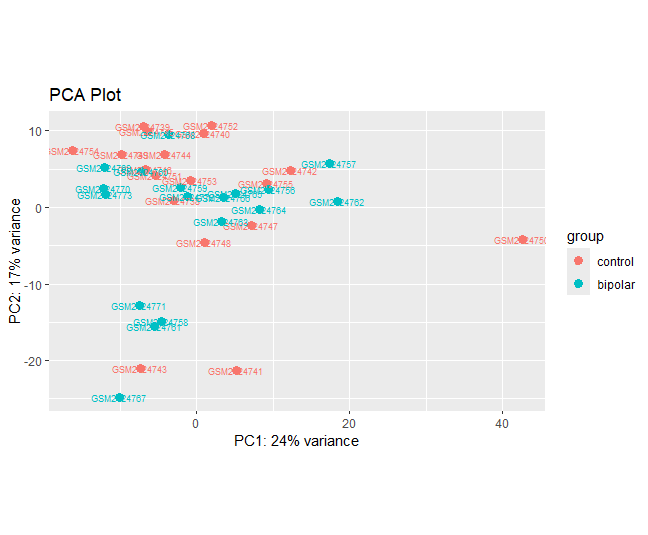
\includegraphics[width=0.7\linewidth]{Plots/PCAPlot.png}
    \caption{PCA Plot}
    \label{fig:PCA_unnormalized}
\end{figure}
In Figure \ref{fig:PCA_unnormalized}, we observe that the two cohorts—control and bipolar—show some degree of clustering, but there exists a partial overlap in the upper-left quadrant. This overlap suggests that while the groups are somewhat distinct, they share biological or technical variability that reduces their separation in the PCA space.  The PCA analysis captures a combined variance of 41{percent-sign} for the first two principal components (PC1 and PC2). This relatively low variance suggests that the underlying variability in the dataset is distributed across multiple dimensions, potentially due to the high dimensionality of the data, biological complexity, or technical noise.  One critical observation is the presence of an outlier, the sample labeled GSM2124750 which corresponds to the control-28 cohort. This sample was flagged as an outlier in the original study \cite{pacifico2017transcriptome}, likely due to either technical artifacts or biological differences that set it apart from the rest of the cohort. Outliers like this can distort PCA results by inflating variance in certain dimensions, thereby reducing the proportion of variance explained by the main principal components.

After removing the outlier from the dataset, we observed a decrease in the variance captured by the first two PCs. The previous study highlighted that clinical variables such as bipolar subtype, medication use, mood state, and other endophenotypes were not known for the bipolar cohort [11], likely contributing to decreased PCA capture. These unaccounted for clinical variables could represent significant sources of heterogeneity within the cohort, further complicating the separation between the control and bipolar groups.

\pagebreak

\section{Differential Gene Expression Analysis}
This section will discuss the implementation and interpretation of differential gene expression (DGE) analysis using the GEO DataSet mentioned above. The following script creates a DESeqData object from the pre-processed raw count matrix and performs the DGE analysis.
\begin{minted}{R}
# Construct DESeqData object from raw count matrix
dds <- DESeqDataSetFromMatrix(countData=counts_data, colData=coldata, design=~ condition)

# Pre-filtering low-count genes
dds <- dds[rowSums(counts(dds)) >= 1, ]

# Set reference level
dds$condition <- relevel(dds$condition, ref = "control")

# Run Differential Gene Expression analysis
dds <- DESeq(dds)
\end{minted}
Then, the following script unpacks the result of the DEG analysis.
\begin{minted}{R}
# Extract and summarize results
res <- results(dds, contrast = c("condition", "control", "bipolar"), alpha = 0.05)
\end{minted}
The \texttt{results} function calculates log2 fold changes, p-values, and adjusted p-values using the Benjamini-Hochberg method for each gene in the provided read count matrix. The contrast argument specifies the comparison of interest; in this case, we are comparing the Bipolar Disorder (BD) condition to the Control (C) condition based on the \texttt{condition} column. The $\alpha$ argument sets the significance threshold to the widely used value of 0.05, which helps control the false discovery rate (FDR). The resulting object, \texttt{res}, contains the differentially expressed genes and their corresponding statistical measures, which will be further analyzed in the subsequent section of the report.

We conducted two separate experiments to assess the impact of an outlier during the quality control process and subsequent differential expression gene (DEG) analysis. Table \ref{table:unnormalized_summary} summarizes the DESeq2 Differential Gene Expression analysis on the original 36-sample GEO DataSet, identifying 12 significant genes. In contrast, Table \ref{table:normalized_summary} summarizes the DESeq2 Differential Gene Expression analysis on the modified GEO DataSet of 35 samples, excluding the outlier control C\_28. This analysis identified 15 significant genes. The increase in significant genes after removing C\_28 supports the authors' claim in \cite{pacifico2017transcriptome} that this control sample is indeed an outlier, as its removal improved the differentiation between the two cohorts, resulting in a greater number of statistically significant genes for comparison.

\begin{table}[H]
\centering
\begin{minipage}{0.45\textwidth}
\centering
\begin{tabular}{lrr}
\toprule
Category & Count & Percentage \\
\midrule
LFC $>$ 0 (up) & 6 & 0.016\% \\
LFC $<$ 0 (down) & 6 & 0.016\% \\
Outliers & 0 & 0\% \\
Low counts & 12374 & 33\% \\
\bottomrule
\end{tabular}
\caption{DEG of original sample}
\label{table:unnormalized_summary}
\end{minipage}
\hspace{10pt}
\begin{minipage}{0.45\textwidth}
\centering
\begin{tabular}{lrr}
\toprule
Category & Count & Percentage \\
\midrule
LFC $>$ 0 (up) & 5 & 0.013\% \\
LFC $<$ 0 (down) & 10 & 0.027\% \\
Outliers & 0 & 0\% \\
Low counts & 5819 & 16\% \\
\bottomrule
\end{tabular}
\caption{DEG of outlier-normalized sample}
\label{table:normalized_summary}
\end{minipage}
\end{table}


\subsection{Dispersion}
DESeq2 offers a valuable criterion known as dispersion to assess whether its negative binomial model is appropriate for the given GEO data. Dispersion quantifies the extent of variation or spread within the dataset. By default, DESeq2 conducts dispersion analysis using a parameter, denoted as $\alpha$, which satisfies the equation $\sigma^2 = \mu + \alpha \dot \mu^2$. In this equation, $\mu$ represents the mean, and $\sigma^2$ denotes the variance of the sample. Figure \ref{fig:unnormalized_Dispersion} presents the dispersion plot.
\begin{figure}[H]
    \centering
    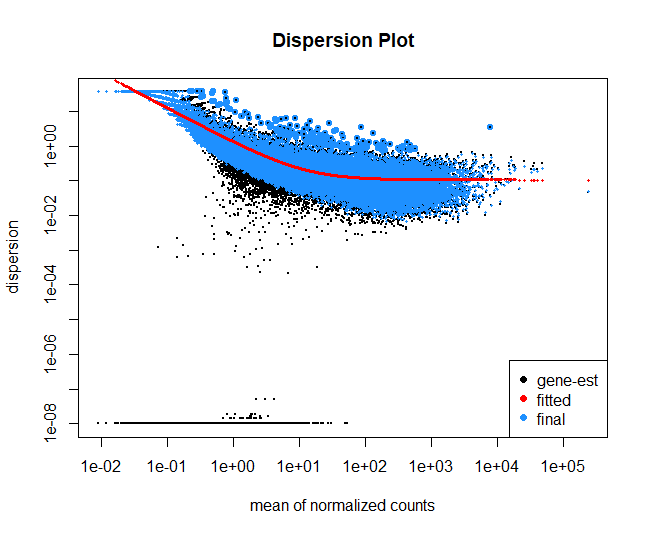
\includegraphics[width=0.4\linewidth]{Plots/DispersionPlot.png}
    \caption{Dispersion Plot}
    \label{fig:unnormalized_Dispersion}
\end{figure}
We can observe that the fitting function is monotonically decreasing. This graph indicates a continuous decrease in dispersion as the mean expression increases. The dispersion estimates generally cluster around the curve, suggesting that the provided GEO DataSet is well-fitted to the DESeq2 model. However, substantial shrinkage is evident due to having only one replicate for each sample in the group.

\subsection{Expression Analysis}
Figure \ref{fig:unnormalized_MA} presents the log fold change MA plot.
\begin{figure}[H]
    \centering
    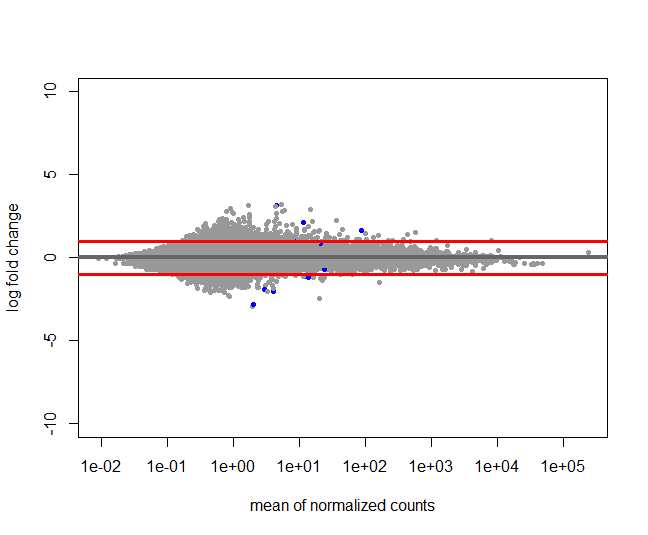
\includegraphics[width=0.4\linewidth]{Plots/MAPlot.png}
    \caption{MA Plot}
    \label{fig:unnormalized_MA}
\end{figure}
This plot visualizes and identifies gene expression changes between two cohorts: "control" and "bipolar" in this case study. The plot displays log fold change (M) on the $y$-axis and the logarithm of the mean normalized gene expression counts for the two conditions on the $x$-axis. 

The plot indicates that genes with lower mean expression values exhibit highly variable log fold changes. The blue dots in Figure \ref{fig:unnormalized_MA} represent differentially expressed genes (DEGs) that have adjusted p-values below the threshold of 0.05. Genes that meet the filtering criteria of a p-value less than 0.05 and a fold change of either greater than 2 (i.e., $\ell>2$) or less than -2 (i.e.,$\ell<-2$) are considered statistically significant. Red vertical lines in the graph mark these thresholds. A fold change greater than 2 (i.e., $\log \ell > 0$) indicates up-regulated genes, while a fold change less than 1 (i.e., $\log \ell < 0$) indicates down-regulated genes. Among the DEGs identified are six up-regulated genes and six down-regulated genes. This analysis is further illustrated in the following plot.
\begin{figure}[H]
    \centering
    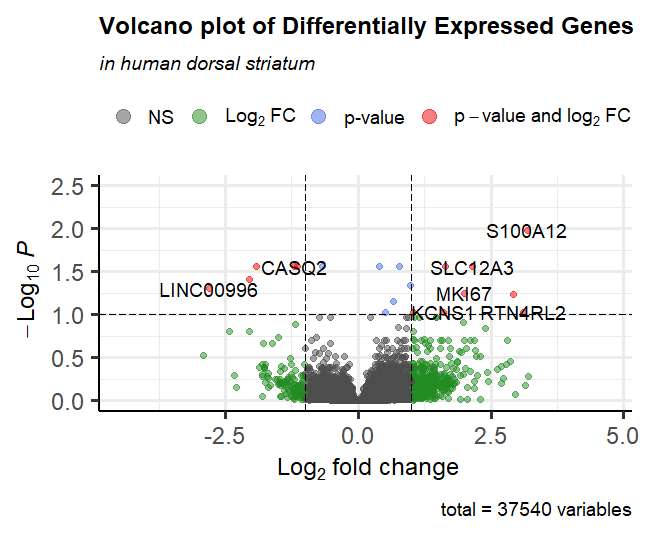
\includegraphics[width=0.5\linewidth]{Plots/VolcanoPlot.png}
    \caption{Volcano plot of DEGs in human dorsal striatum}
    \label{fig:volcano_unnormalized}
\end{figure}
To further analyze the functions of the statistically significant differentially expressed genes, we paired each gene with the reference database provided by the R library \texttt{org.Hs.eg.db}. This library offers mappings between Entrez Gene identifiers and GenBank accession numbers, including Ensemble IDs. Figure \ref{fig:volcano_unnormalized} illustrates the volcano plot of differentially expressed genes. Statistically significant genes are highlighted in red on the plot. Among these, genes with positive log fold changes are considered up-regulated. Table \ref{table:up_regulated} provides a comprehensive list of the up-regulated genes depicted in the volcano plot, along with additional details.
\begin{table}[H]
    \centering
    \begin{tabular}{rrrrrrrrl}
    \toprule
    ENSG ID & baseMean & log2FoldChange & lfcSE & stat & pvalue & padj & symbol \\
    \midrule
    00000070915 & 11.471846 & 2.156212 & 0.487764 & -4.420603 & 9.8426e-06 & 0.0275 & SLC12A3 \\
    00000124134 & 19.494935 & 1.609598 & 0.403496 & -3.989133 & 6.6315e-05 & 0.0927 & KCNS1 \\
    00000148773 & 7.761059 & 2.001743 & 0.478666 & -4.181919 & 2.8905e-05 & 0.0559 & MKI67 \\
    00000163221 & 4.440045 & 3.184795 & 0.629121 & -5.062293 & 4.1424e-07 & 0.0104 & S100A12 \\
    00000165985 & 14.377425 & 2.915072 & 0.700847 & -4.159356 & 3.1914e-05 & 0.0573 & C1QL3 \\
    00000186907 & 4.295899 & 3.110264 & 0.782409 & -3.975241 & 7.0308e-05 & 0.0931 & RTN4RL2 \\
    00000198743 & 1185.410114 & 1.034511 & 0.258776 & -3.997709 & 6.3958e-05 & 0.0927 & SLC5A3 \\
    00000275395 & 87.451458 & 1.643967 & 0.359915 & -4.567649 & 4.9322e-06 & 0.0275 & FCGBP \\
    \bottomrule
    \end{tabular}
    \caption{Complete List of up-regulated genes}
    \label{table:down_regulated}
\end{table}
Some up-regulated genes are associated with immune responses, transmembrane transport, and protein-coding and non-protein-coding functions.

First, SLC12A3, also known as solute carrier family 12 member 3, encodes the sodium-chloride cotransporter (NCC), crucial for sodium and chloride ion reabsorption in the kidney's distal convoluted tubules. The gene’s function in regulating ion homeostasis, cell volume, and neuronal excitability has been well-documented \cite{Zhang2023Role, Li2022Gitelman, Trejo2023CryoEM}. Up-regulation of SLC12A3 is predicted to disrupt these processes, with implications for conditions like Gitelman syndrome \cite{Li2022Gitelman}.

Next, KCNS1, or potassium voltage-gated channel subfamily S member 1, encodes a modulatory subunit that forms heteromultimers with other potassium channels to regulate neuronal excitability and synaptic function. Its up-regulation has been associated with altered synaptic transmission \cite{Koch2020Potassium}. MKI67, a marker for cell proliferation, plays a role in chromosomal organization during mitosis. Up-regulation of MKI67 has been linked to reduced cell division, often serving as a marker for low proliferative activity in cells \cite{Rahman2015Ki67}.

The S100A12 gene encodes calgranulin C, a calcium-binding protein involved in immune response and inflammation. By regulating calcium-dependent processes, including muscle contraction and neuronal signaling, up-regulation may impair immune responses and antibacterial properties \cite{Foell2007S100}.

The role of C1QL3 remains incompletely understood but is linked to immune regulation and inflammation. Similarly, RTN4RL2 is critical for neuronal development and plasticity; its up-regulation correlates strongly with bipolar disorder pathology \cite{Smith2019Neurodevelopment}.

Finally, SLC5A3, encoding a sodium/glucose co-transporter, is essential for glucose uptake and metabolism. Up-regulation impairs glucose metabolism, highlighting its role in cellular energy homeostasis \cite{Chen2019SLC5A}. Lastly, FCGBP, involved in lipid metabolism, remains under explored, though its up-regulation is hypothesized to affect lipid regulation and energy balance \cite{Kim2020Lipids}.

Similarly, the genes exhibiting negative log fold changes are classified as down-regulated. Table \ref{table:down_regulated} provides a complete list of these down-regulated genes, which are represented in the volcano plot, along with additional details.

\begin{table}[H]
    \centering
    \begin{tabular}{rrrrrrrrl}
    \toprule
    ENSG ID & baseMean & log2FoldChange & lfcSE & stat & pvalue & padj & symbol \\
    \midrule
    00000118729 & 13.395064 & -1.199622 & 0.263730 & 4.548668 & 5.3986e-06 & 0.0275 & CASQ2 \\
    00000132744 & 3.952897 & -2.052703 & 0.475144 & 4.320168 & 1.5591e-05 & 0.0392 & ACY3 \\
    00000144681 & 12.769351 & -1.141231 & 0.251624 & 4.535454 & 5.7479e-06 & 0.0275 & STAC \\
    00000239961 & 2.897106 & -1.917298 & 0.431810 & 4.440140 & 8.9900e-06 & 0.0275 & LILRA4 \\
    00000242258 & 2.019025 & -2.799696 & 0.662369 & 4.226795 & 2.3704e-05 & 0.0497 & LINC00996 \\
    \bottomrule
    \end{tabular}
    \caption{Complete list of up-regulated genes}
    \label{table:down_regulated}
\end{table}
Many down-regulated genes are involved in ion transport, cell proliferation, and calcium signaling. 

Firstly, the LILRA4 gene encodes an immunoglobulin-like protein found on the surface of plasmacytoid dendritic cells (pDCs), a rare immune cell subset specialized in antiviral responses and the production of type I interferons \cite{Lim2023LILRA4, Palma2012LILRA4}. Its expression enhances immune regulation, contributing to the innate and adaptive immune response, including during viral infections and inflammatory diseases \cite{Kioon2024LILRA4, Yun2021LILRA4}.

Secondly, the ACY3 gene, also known as aminoacylase 3, encodes a protein critical for deacetylating mercapturic acids in the proximal tubules of the kidney. This gene plays a significant role in maintaining renal function and detoxification processes \cite{Jones2020ACY3}. Additionally, LINC00996, a long intergenic non-coding RNA, has been shown to suppress the migration, invasion, and proliferation of lung adenocarcinoma cells, indicating its role in tumor suppression and cellular homeostasis \cite{Wang2018LINC00996}.

Calsequestrin 2 (CASQ2), a high-capacity calcium-binding protein, functions as an internal calcium reservoir within muscle tissues. It is pivotal in regulating calcium homeostasis, influencing muscle contraction and relaxation cycles \cite{Park2019CASQ2}. Lastly, the STAC gene encodes a scaffold protein that modulates calcium channel expression and function. STAC enhances the activity of calcium channels such as CACNA1H and CACNA1S and slows the inactivation of CACNA1C, which is critical for maintaining cellular calcium signaling \cite{Lopez2021STAC}.

Figure \ref{fig:unnormalized_heatmaps} (a) and (b) illustrate heatmaps depicting sample-to-sample distances and the counts of significant differentially expressed genes (DEGs).
\begin{figure}[H]
    \centering
    \subfloat[\centering Heatmap of pairwise distances among samples]{{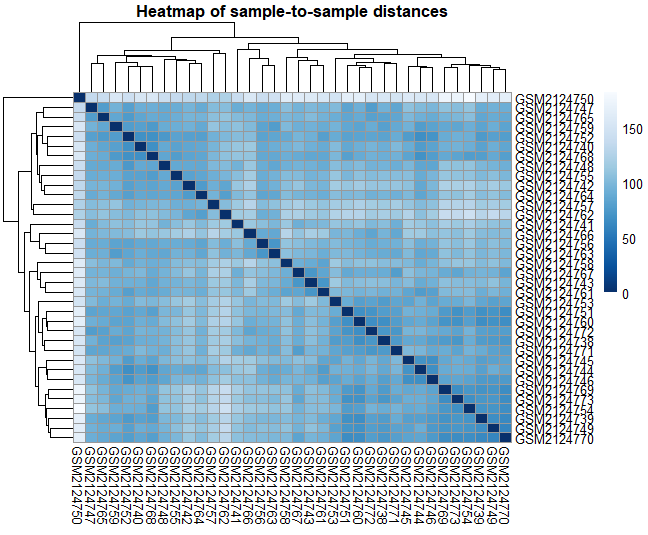
\includegraphics[width=8cm]{Plots/HeatmapPairwisePlot.png} }}%
    \qquad
    \subfloat[\centering Heatmap of significant DEGs]{{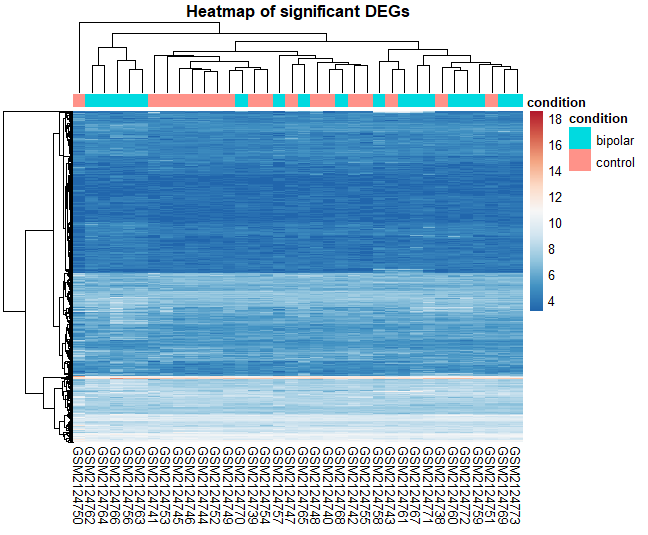
\includegraphics[width=8cm]{Plots/HeatmapDEGPlot.png} }}%
    \caption{Heatmap Plots}
    \label{fig:unnormalized_heatmaps}
\end{figure}
In figure \ref{fig:unnormalized_heatmaps} (a), the correlation heatmap and dendrogram represent all 36 samples based on the Euclidean distances calculated from expression data for all genes. The sample labeled GSM2124750, corresponding to C\_28, was identified as an outlier in the original study \cite{pacifico2017transcriptome}. The heatmap and the dendrogram indicate that it is an outlier. The heatmap aligns with the findings of the original study. Additionally, among the 12 differentially expressed genes identified between groups, some are known immune effectors, with two previously linked to neuropsychiatric disorders.

As a similar study was conducted using the exact same raw sample data, notable differences have emerged in the differentially expressed genes (DEGs) between the two analyses. While our analysis identified several unique DEGs that were not reported in the previous study, there were also genes present in the previous study that are absent from ours.


\begin{table}[H]
    \centering
    \begin{tabular}{llll}
        \toprule
        \text{Ensembl ID}& \text{Gene}& \text{Type of Gene}& \text{Expression Status}\\ 
        \midrule
        00000132744         & ACY3          & Protein-coding        & Under-expressed \\ 
        00000070915         & SLC12A3       & Protein-coding        & Over-expressed  \\ 
        00000124134         & KCNS1         & Protein-coding        & Over-expressed  \\ 
        00000148773         & MKI67         & Protein-coding        & Over-expressed  \\ 
        00000165985         & C1QL3         & Protein-coding        & Over-expressed  \\ 
        00000186907         & RTN4RL2       & Protein-coding        & Over-expressed  \\ 
        00000198743         & SLC5A3        & Protein-coding        & Over-expressed  \\ 
        \bottomrule
    \end{tabular}
    \caption{Genes Absent from Past Study}
    \label{tab:unique_genes}
\end{table}

\begin{table}[H]
    \centering
    \begin{tabular}{llll}
        \toprule
        Ensembl ID          & Gene               & Type of Gene            & Expression Status         \\ 
        \midrule
        ENSG00000253661     & ZFHX4-AS1          & Antisense               & Under-expressed           \\ 
        ENSG00000260912     & RP11-363E7.4       & Sense overlap           & Over-expressed            \\ 
        ENSG00000260064     & RP11-18F14.4       & Sense intronic          & Over-expressed            \\ 
        ENSG00000240032     & RP11-274H2.3       & Antisense               & Over-expressed            \\ 
        ENSG00000219665     & CTD-2006C1.2       & Proc. transcript        & Over-expressed            \\ 
        ENSG00000156219     & ART3               & Protein-coding          & Under-expressed           \\ 
        ENSG00000140853     & NLRC5              & Protein-coding          & Over-expressed            \\ 
        ENSG00000099968     & BCL2L13            & Protein-coding          & Over-expressed            \\ 
        \bottomrule
    \end{tabular}
    \caption{Genes Absent from Our Analysis but Present in Past Study}
    \label{tab:absent_genes}
\end{table}

Some potential factors that may have contributed to the identification of these unique genes include variations in the analytical frameworks used during pipeline development, as well as differences in preprocessing, normalization techniques, and statistical analysis methodologies. Differences in gene annotation databases across studies, particularly in identifying antisense, sense overlap, or protein-coding transcripts, may also explain these variations.

\pagebreak

\section{Conclusion}
\subsection{Problems}
The first challenge encountered was the substantial computational requirements of the pre-processing procedures. Raw FASTQ files generated by the Illumina HiSeq RNA-Seq platform ranged in size from 2–6 GB each. With a total of 36 files to download and process, this necessitated considerable memory and disk space to execute tools such as HISAT2 and htseq-count effectively. Processing locally was not feasible, so we had to gain access to the  Cedar heterogeneous cluster at Simon Fraser University to accommodate the computational demands.

Another significant challenge was the complexity of the preprocessing workflow. Multiple software tools and frameworks were required to prepare the data for downstream analysis. For example, HISAT2 was used to align the reads to the reference genome, and htseq-count was used to quantify feature-level counts. This multi-step process added a layer of intricacy to the analysis pipeline.

Additionally, the need to source data from multiple repositories introduced potential risks to the integrity and consistency of the analysis. For instance, the cohort dataset was obtained from the NCBI Sequence Read Archive (SRA), while the Homo sapiens gene annotation file (GFF format) was sourced from the NCBI Homo sapiens database. Discrepancies between data versions or inconsistencies across sources could compromise the accuracy and reliability of the results, underscoring the importance of rigorous version control and cross-validation during data acquisition.

\subsection{Findings}
To conclude the report, we will summarize the results of the analysis. In this study, we profiled transcriptomes using RNA-Seq data from the human dorsal striatum, comparing cohorts of patients with bipolar disorder (BD) to control subjects. We utilized the \texttt{DESeq2} library to perform differential gene expression (DGE) analysis, aiming to identify changes in gene expression associated with bipolar disorder status. 

The results were further analyzed to identify sets of correlated genes that show an association with bipolar disorder. Through our DGE analysis, we identified several immune response genes, such as S100A12, LILRA4, and FCGBP, as well as various non-protein coding genes. Unlike the original study, we did not identify the immune response gene NLRC5 in our analysis. As well as several other sense genes that were not captured as statistically over- or under-expressed within our threshold.

Some potential factors that may have contributed to the differing results include variations in frameworks employed during the development of the pipeline, as well as differences in preprocessing and analysis methodologies. Additionally, while the original study \cite{pacifico2017transcriptome} reported that fourteen genes were differentially expressed at a 5\% false discovery rate, our analysis, which included the outlier C\_28 control sample, revealed only thirteen genes as differentially expressed at a 10\% false discovery rate. 

\pagebreak
\printbibliography[
heading=bibintoc,
title={Bibliography}]

\end{document}
